\documentclass[10pt,mathserif]{beamer}

\usepackage{graphicx,amsmath,amssymb}
\usepackage{subcaption, natbib, hyperref}
\hypersetup{
    colorlinks=true,
    linkcolor=blue,
    filecolor=magenta,
    urlcolor=cyan,
}

% ------------------------------------------------------------------------
% Packages
% ------------------------------------------------------------------------
\usepackage{amsmath}

% ------------------------------------------------------------------------
% Macros
% ------------------------------------------------------------------------
%~~~~~~~~~~~~~~~
% List shorthand
%~~~~~~~~~~~~~~~
\newcommand{\BIT}{\begin{itemize}}
\newcommand{\EIT}{\end{itemize}}
\newcommand{\BNUM}{\begin{enumerate}}
\newcommand{\ENUM}{\end{enumerate}}
%~~~~~~~~~~~~~~~
% Text with quads around it
%~~~~~~~~~~~~~~~
\newcommand{\qtext}[1]{\quad\text{#1}\quad}
%~~~~~~~~~~~~~~~
% Shorthand for math formatting
%~~~~~~~~~~~~~~~
\newcommand\mbb[1]{\mathbb{#1}}
\newcommand\mbf[1]{\mathbf{#1}}
\def\mc#1{\mathcal{#1}}
\def\mrm#1{\mathrm{#1}}
%~~~~~~~~~~~~~~~
% Common sets
%~~~~~~~~~~~~~~~
\def\reals{\mathbb{R}} % Real number symbol
\def\integers{\mathbb{Z}} % Integer symbol
\def\rationals{\mathbb{Q}} % Rational numbers
\def\naturals{\mathbb{N}} % Natural numbers
\def\complex{\mathbb{C}} % Complex numbers
\def\simplex{\mathcal{S}} % Simplex
%~~~~~~~~~~~~~~~
% Common functions
%~~~~~~~~~~~~~~~
\renewcommand{\exp}[1]{\operatorname{exp}\left(#1\right)} % Exponential
\def\indic#1{\mbb{I}\left({#1}\right)} % Indicator function
\providecommand{\argmax}{\mathop\mathrm{arg max}} % Defining math symbols
\providecommand{\argmin}{\mathop\mathrm{arg min}}
\providecommand{\arccos}{\mathop\mathrm{arccos}}
\providecommand{\asinh}{\mathop\mathrm{asinh}}
\providecommand{\dom}{\mathop\mathrm{dom}} % Domain
\providecommand{\range}{\mathop\mathrm{range}} % Range
\providecommand{\diag}{\mathop\mathrm{diag}}
\providecommand{\tr}{\mathop\mathrm{tr}}
\providecommand{\abs}{\mathop\mathrm{abs}}
\providecommand{\card}{\mathop\mathrm{card}}
\providecommand{\sign}{\mathop\mathrm{sign}}
\def\rank#1{\mathrm{rank}({#1})}
\def\supp#1{\mathrm{supp}({#1})}
%~~~~~~~~~~~~~~~
% Common probability symbols
%~~~~~~~~~~~~~~~
\def\E{\mathbb{E}} % Expectation symbol
\def\Earg#1{\E\left[{#1}\right]}
\def\Esubarg#1#2{\E_{#1}\left[{#2}\right]}
\def\P{\mathbb{P}} % Probability symbol
\def\Parg#1{\P\left({#1}\right)}
\def\Psubarg#1#2{\P_{#1}\left[{#2}\right]}
\def\Cov{\mrm{Cov}} % Covariance symbol
\def\Covarg#1{\Cov\left[{#1}\right]}
\def\Covsubarg#1#2{\Cov_{#1}\left[{#2}\right]}
\def\Var{\mrm{Var}}
\def\Vararg#1{\Var\left(#1\right)}
\def\Varsubarg#1#2{\Var_{#1}\left(#2\right)}
\newcommand{\family}{\mathcal{P}} % probability family
\newcommand{\eps}{\epsilon}
\def\absarg#1{\left|#1\right|}
\def\msarg#1{\left(#1\right)^{2}}
\def\logarg#1{\log\left(#1\right)}
%~~~~~~~~~~~~~~~
% Distributions
%~~~~~~~~~~~~~~~
\def\Gsn{\mathcal{N}}
\def\Ber{\textnormal{Ber}}
\def\Bin{\textnormal{Bin}}
\def\Unif{\textnormal{Unif}}
\def\Mult{\textnormal{Mult}}
\def\Cat{\textnormal{Cat}}
\def\Gam{\textnormal{Gam}}
\def\InvGam{\textnormal{InvGam}}
\def\NegMult{\textnormal{NegMult}}
\def\Dir{\textnormal{Dir}}
\def\Lap{\textnormal{Laplace}}
\def\Bet{\textnormal{Beta}}
\def\Poi{\textnormal{Poi}}
\def\HypGeo{\textnormal{HypGeo}}
\def\GEM{\textnormal{GEM}}
\def\BP{\textnormal{BP}}
\def\DP{\textnormal{DP}}
\def\BeP{\textnormal{BeP}}
%~~~~~~~~~~~~~~~
% Theorem-like environments
%~~~~~~~~~~~~~~~

%-----------------------
% Probability sets
%-----------------------
\newcommand{\X}{\mathcal{X}}
\newcommand{\Y}{\mathcal{Y}}
\newcommand{\D}{\mathcal{D}}
\newcommand{\Scal}{\mathcal{S}}
%-----------------------
% vector notation
%-----------------------
\newcommand{\bx}{\mathbf{x}}
\newcommand{\by}{\mathbf{y}}
\newcommand{\bt}{\mathbf{t}}
\newcommand{\xbar}{\overline{x}}
\newcommand{\Xbar}{\overline{X}}
\newcommand{\tolaw}{\xrightarrow{\mathcal{L}}}
\newcommand{\toprob}{\xrightarrow{\mathbb{P}}}
\newcommand{\laweq}{\overset{\mathcal{L}}{=}}
\newcommand{\F}{\mathcal{F}}
\def\colarg#1#2{\textcolor[HTML]{#1}{#2}}


\mode<presentation>
{
\usetheme{default}
}
\setbeamertemplate{navigation symbols}{}
\usecolortheme[rgb={0.13,0.28,0.59}]{structure}
\setbeamertemplate{itemize subitem}{--}
\setbeamertemplate{frametitle} {
	\begin{center}
	  {\large\bf \insertframetitle}
	\end{center}
}

\AtBeginSection[]
{
	\begin{frame}<beamer>
		\frametitle{Outline}
		\tableofcontents[currentsection,currentsubsection]
	\end{frame}
}

%% begin presentation

\title{\large \bfseries Humanitarian AI Roundtable \\ Crisis Mapping and Super-Resolution}

\author{Kris Sankaran and Pablo Fonseca\\ (Work with Rifat Arefin, Anthony
  Ortiz, Jason Jo, Vincent Michalski, and Samira Kahou)}

\date{\today}

\begin{document}
\maketitle

%% \begin{frame}
%%   \frametitle{Maps are Useful}
%%   Especially if you have a critical mission.
%%  \begin{figure}[ht]
%%    \centering
%%    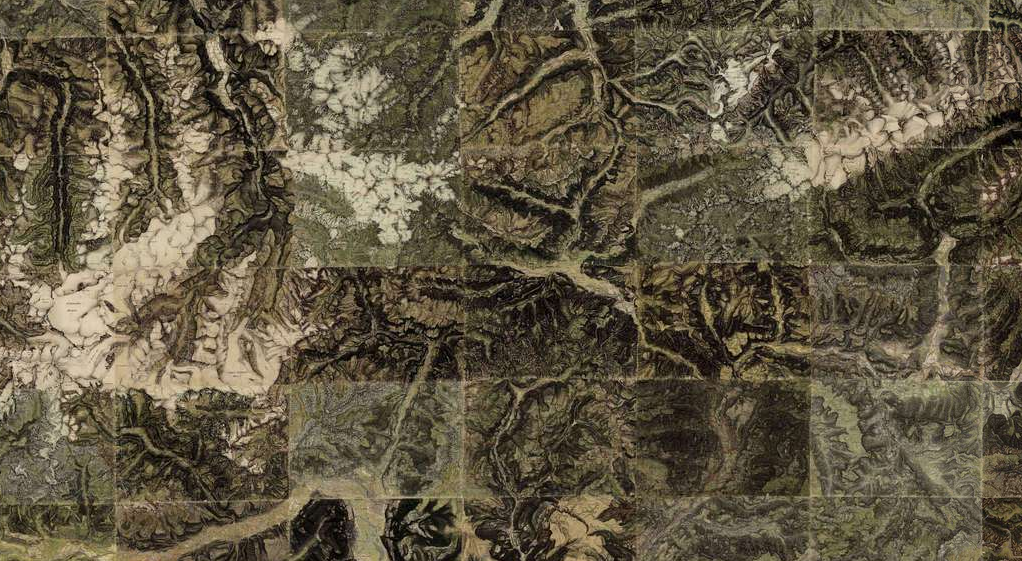
\includegraphics[width=0.6\paperwidth]{figures/old_map}
%%    \caption{A mapping of Tyrol, from the Second Military Survey of the Habsburg
%%      Empire.\label{fig:label} }
%%  \end{figure}
%% \end{frame}

%% \begin{frame}
%%   \frametitle{Maps are Useful}
%%  \begin{figure}[ht]
%%    \centering
%%    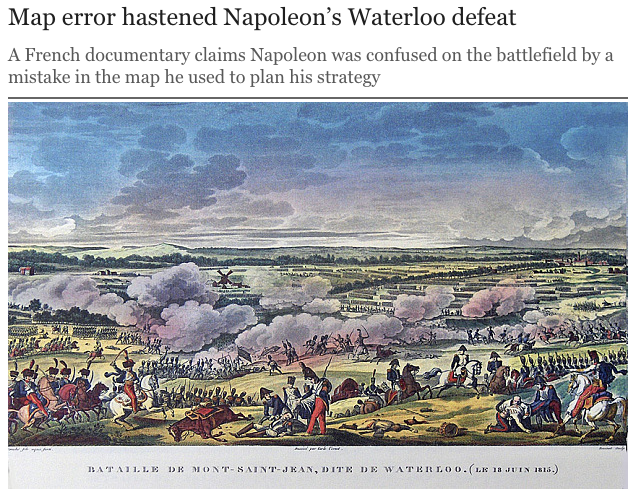
\includegraphics[width=0.6\paperwidth]{figures/napoleon_map}
%%    \caption{This is what false positives look like.}
%%  \end{figure}
%% \end{frame}

\begin{frame}
  \frametitle{Improving Sensing}
  \begin{itemize}
  \item Map Annotation
    \begin{itemize}
    \item How to augment human volunteers, and scale annotations?
    \item Use case: Pandemic response planning
    \end{itemize}
  \end{itemize}
  \begin{figure}
    \centering
    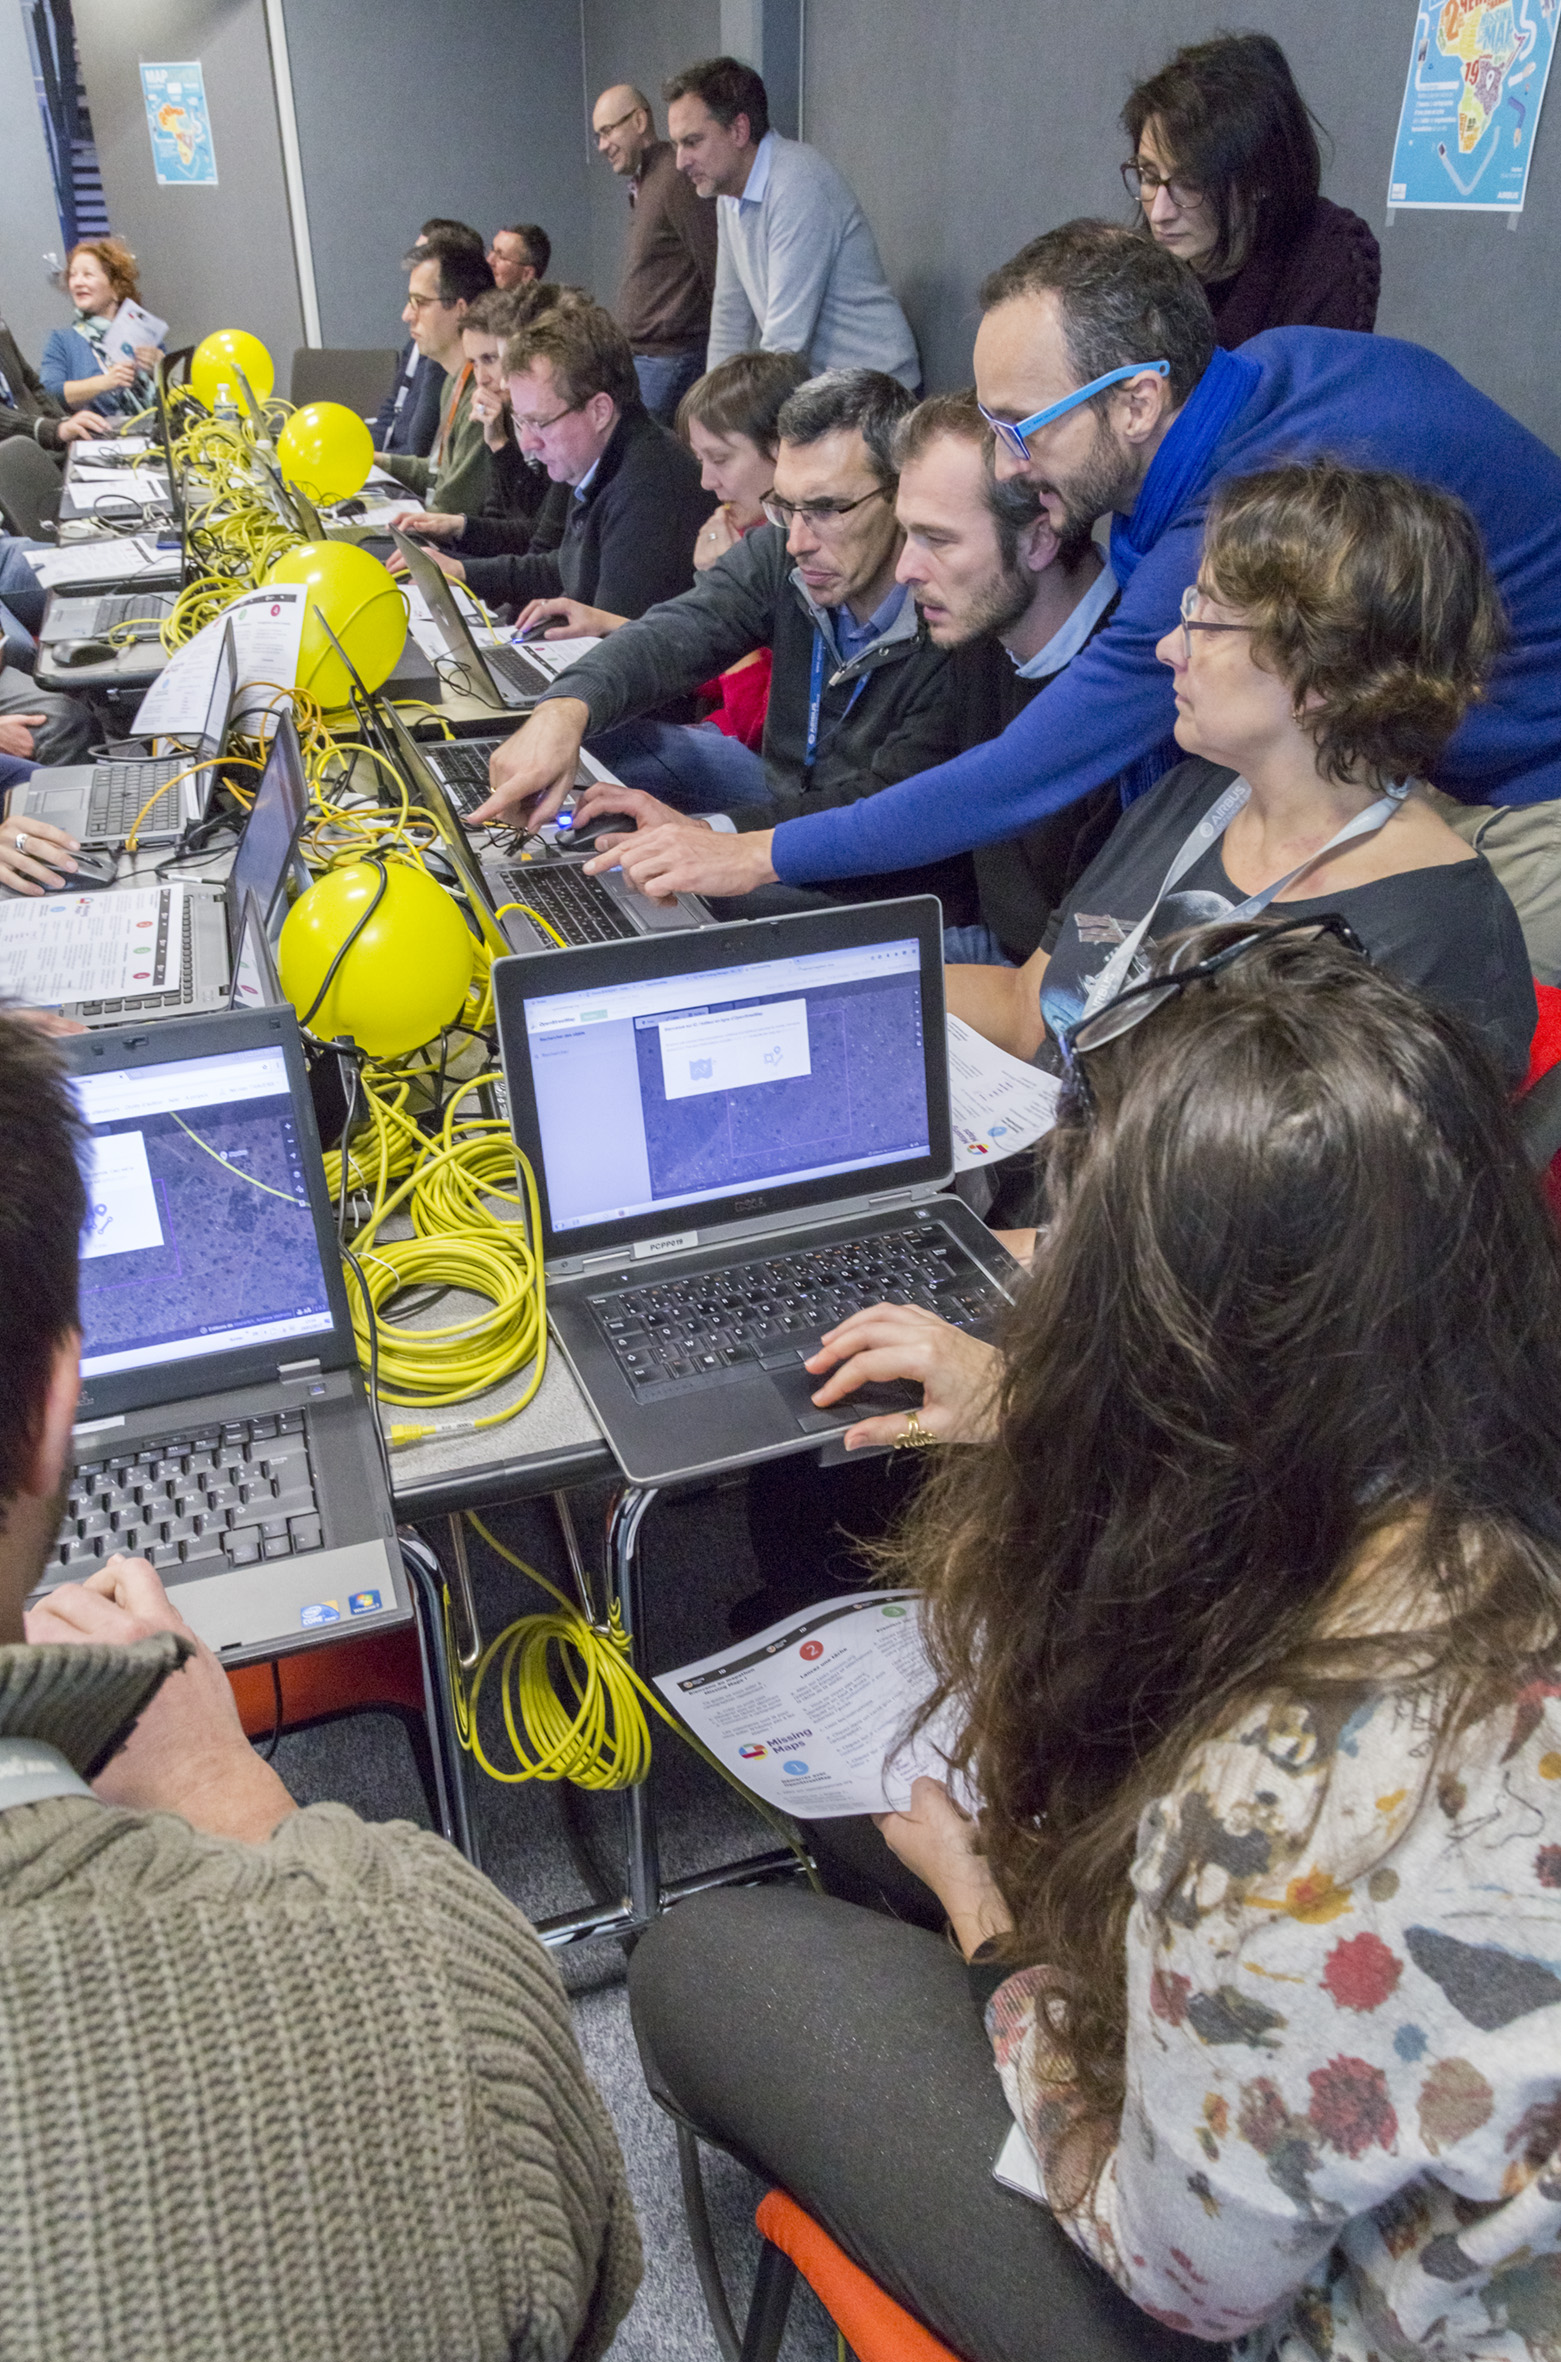
\includegraphics[width=0.3\paperwidth]{figures/mapathon}
    \caption{Exampling crowdsourcing session, from the MissingMaps
      websie. \label{fig:label} }
  \end{figure}
\end{frame}

\begin{frame}
  \frametitle{Research Problems: Map Annotation}
  \begin{itemize}
  \item \textbf{Conditional U-Net}: Models robust across a variety of environments
  \item \textbf{Interactive Corrections}: Leverage human volunteers efficiently
  \item \textbf{Useable Uncertainties}: Streamline validation and correction processes
  \item \textbf{Incremental Annotations}: Learn across a hierarchy of annotations
  \end{itemize}  
  \begin{figure}[ht]
    \centering
    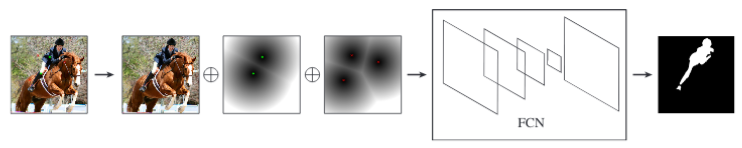
\includegraphics[width=0.85\paperwidth]{figures/classical_interactive}
    \caption{One approach to more interactive image segmentation, from ``Deep
      Object Selection.'' \label{fig:label} }
  \end{figure}
\end{frame}

\begin{frame}
  \frametitle{Improving Sensing}
  \begin{itemize}
  \item Super-Resolution
    \begin{itemize}
    \item How to end monopolies on high-res maps?
    \item Use case: Quantifying extent of violence in Darfur
    \end{itemize}
  \end{itemize} 
  \begin{figure}[ht]
    \centering
    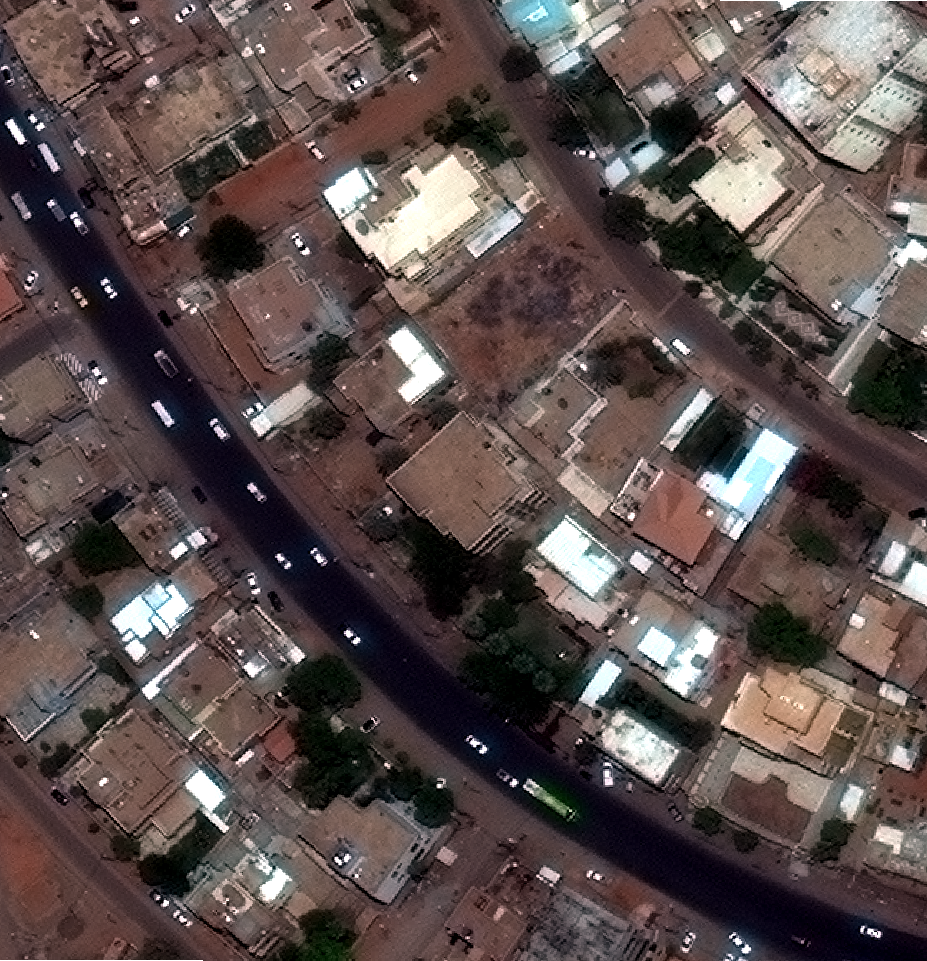
\includegraphics[width=0.4\paperwidth]{figures/high_res_khartoum}
    \caption{A high-resolution image of a street in Khartoum. \label{fig:label} }
  \end{figure}
\end{frame}

\begin{frame}
  \begin{itemize}
  \item Super-Resolution
    \begin{itemize}
    \item How to end monopolies on high-res satellite images?
    \item Use case: Quantifying extent of violence in Darfur
    \end{itemize}
  \end{itemize} 
  \begin{figure}[ht]
    \centering
    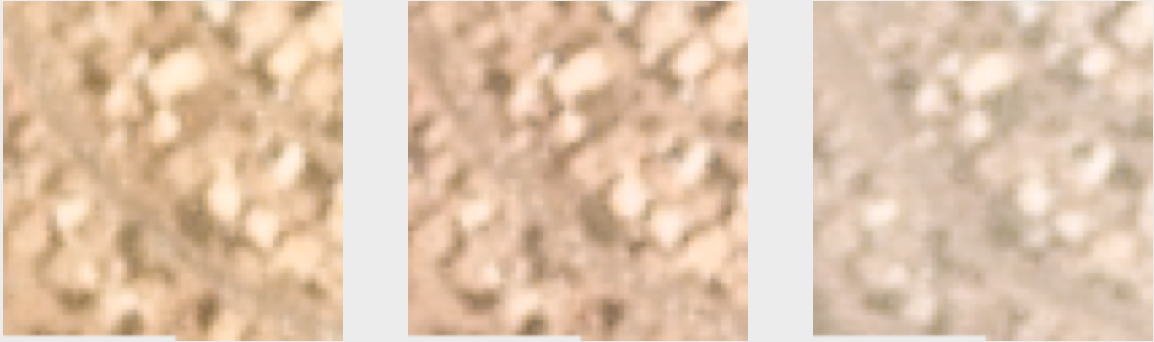
\includegraphics[width=0.8\paperwidth]{figures/multiframe_khartoum}
    \caption{Corresponding low-res views. \label{fig:label} }
  \end{figure}
\end{frame}

\begin{frame}
  \begin{itemize}
  \item Super-Resolution
    \begin{itemize}
    \item How to end monopolies on high-res satellite images?
    \item Use case: Quantifying extent of violence in Darfur
    \end{itemize}
  \end{itemize} 
  \begin{figure}[ht]
    \centering
    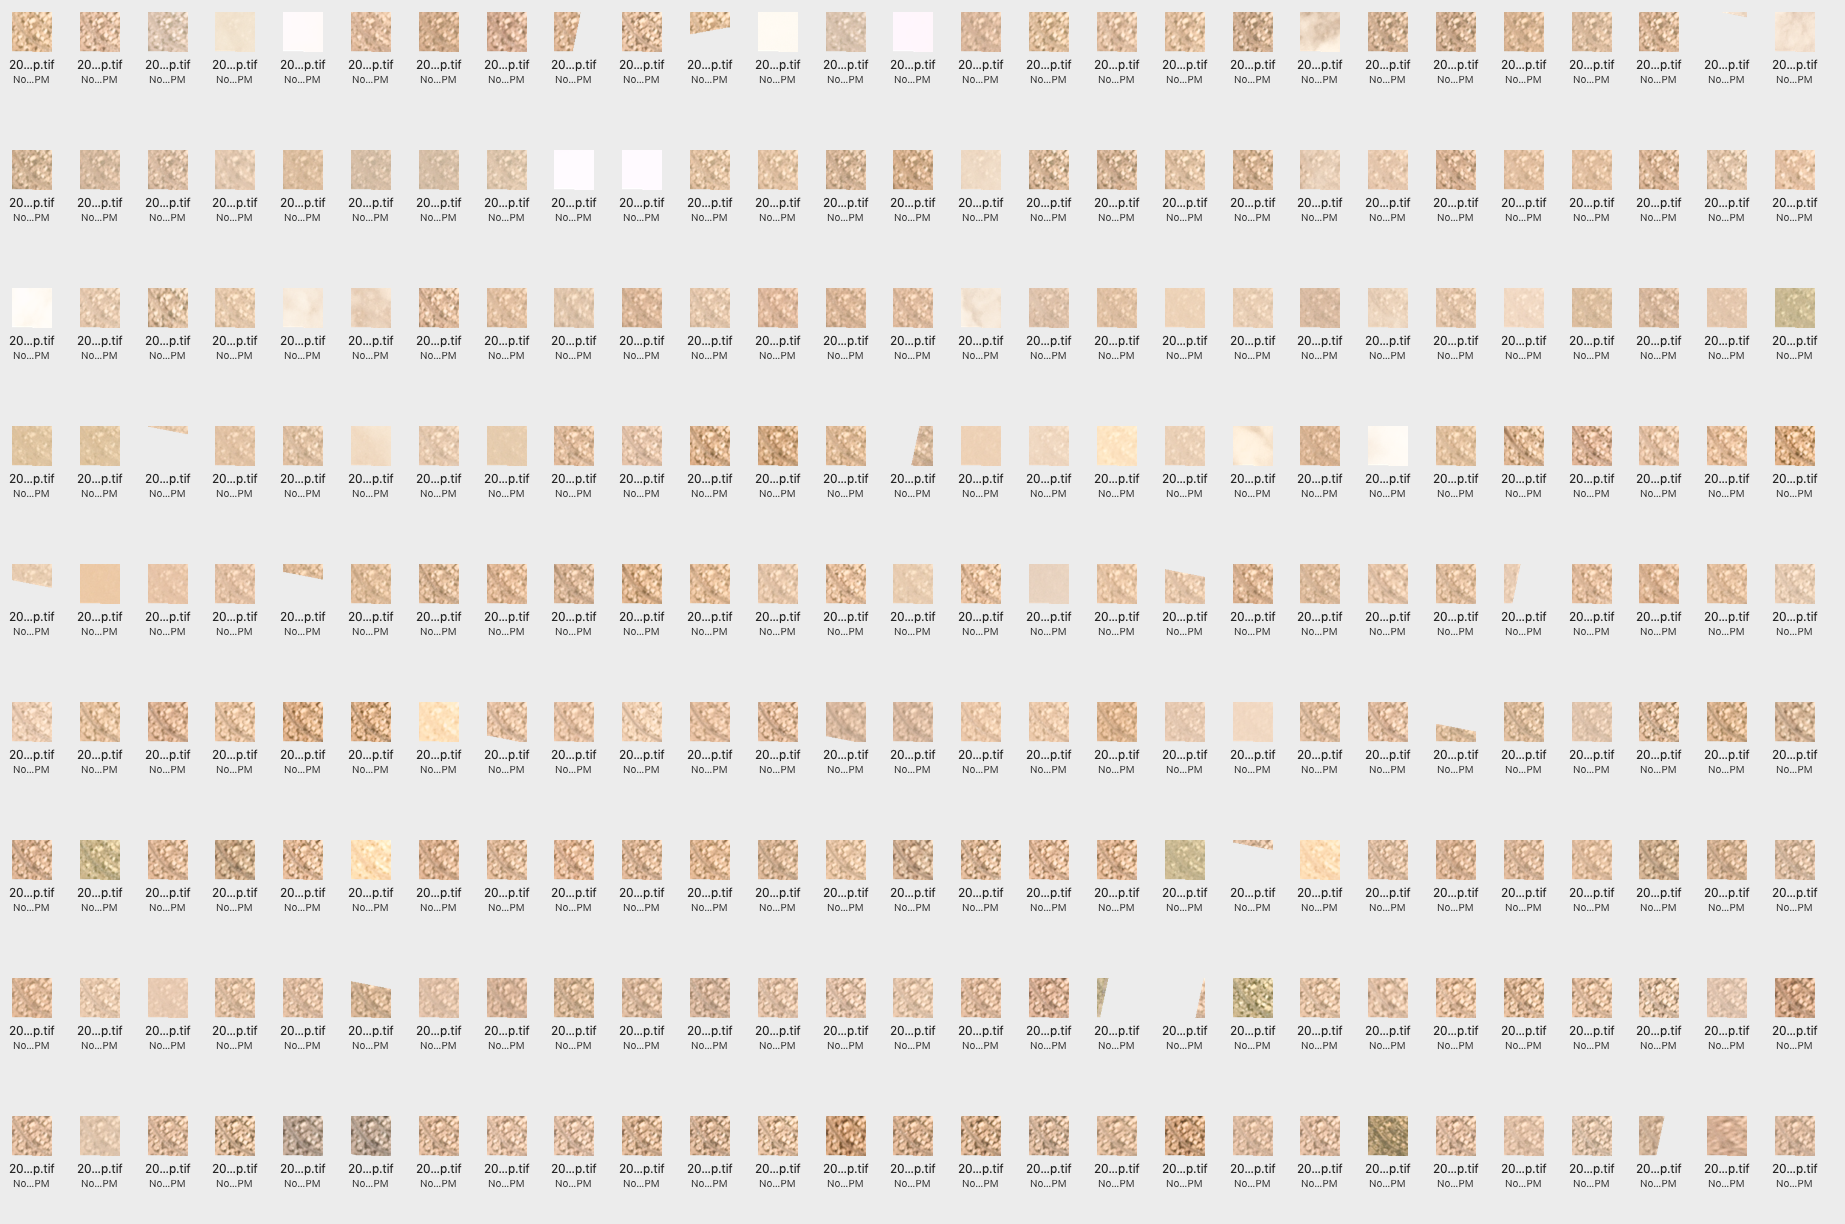
\includegraphics[width=0.7\paperwidth]{figures/multliframe_khartoum_2}
    \caption{Corresponding low-res views. \label{fig:label} }
  \end{figure}
\end{frame}

\begin{frame}
  \frametitle{Research Problems: Super-Resolution}
  \begin{itemize}
  \item Conditioning: How to incorporate metadata into super-resolution?
  \item Multiframedness: Dealing with alignment and using multiple inputs
    (Knowledge Graphs, multichannel, and recurrence)
  \end{itemize}
  \begin{figure}[ht]
    \centering
    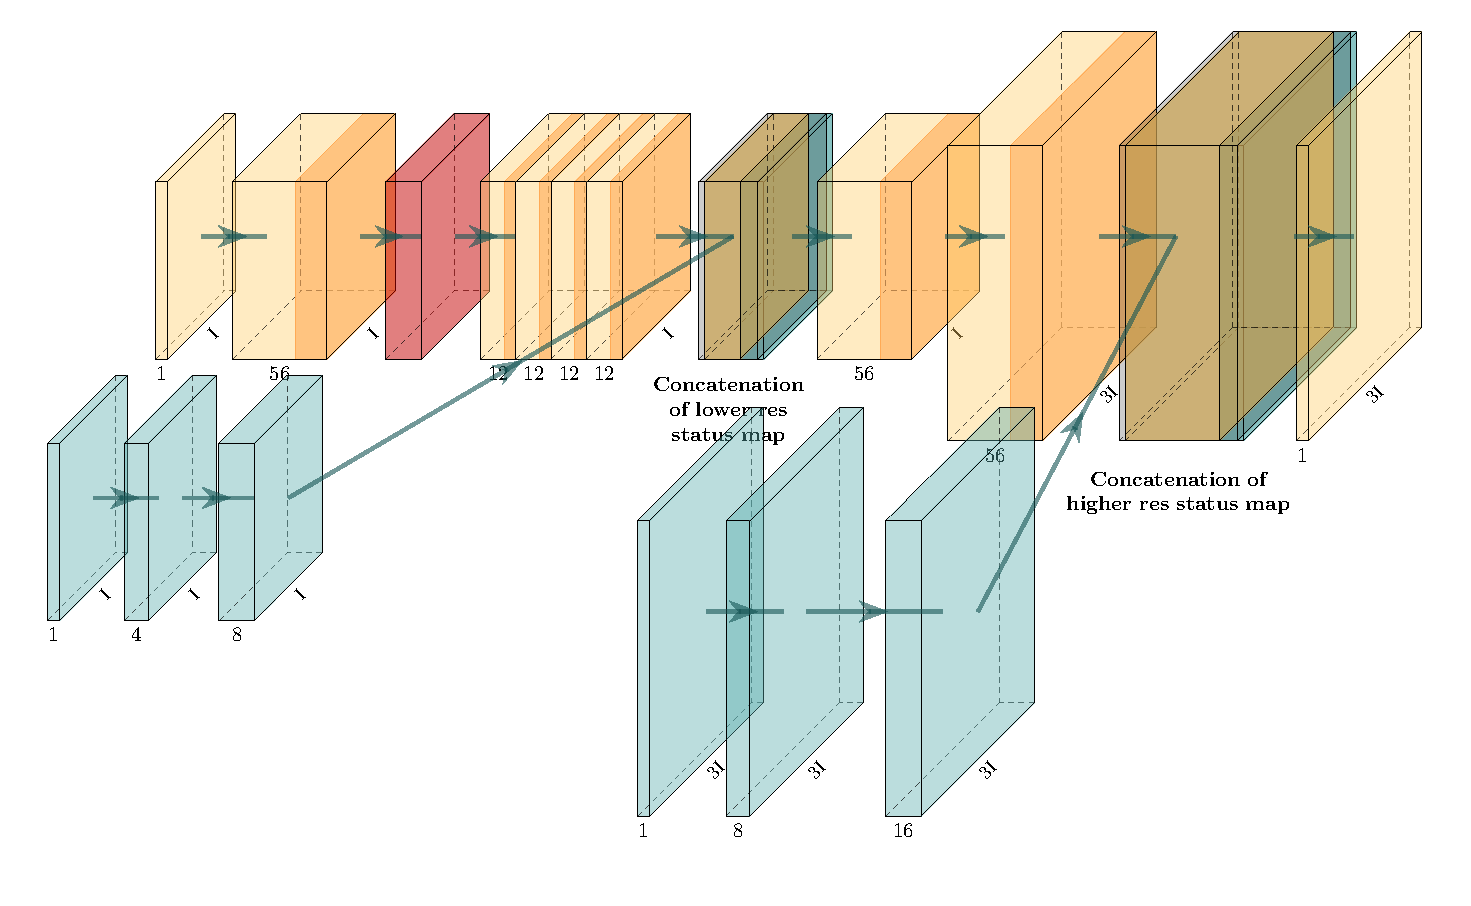
\includegraphics[width=0.6\paperwidth]{figures/conditioning_network}
    \caption{Example of conditioning architecture used for super-resolution. \label{fig:label} }
\end{figure}


\end{frame}

\begin{frame}
  \frametitle{Challenges}
  \begin{itemize}
  \item Narrowing on problems -- schools or bridges? Myanmar or Uganda?
  \item Getting data!
  \item Abstractions vs. applications
  \end{itemize}
\end{frame}

\begin{frame}
  \frametitle{Lessons Learned}
  \begin{itemize}
  \item Decide on your own MNIST
  \item Define intermediate successes
  \item There are more venues than you think
  \end{itemize}
\end{frame}

\end{document}
